\chapter{Theory}
\label{ch:2}

This section is largely based on the work done for the course \textit{TDT4501 Computer Science, Specialization Project}\cite{0-SimilarityMeasures}. 
It is assumed that the readers of this thesis will not have read the final report and thus some of its content is restated. 
This chapter aims to summarize the related to trajectories and the manners of computing their similarity.
We define terms and notation that will be used throughout this work and close the chapter by providing background for trajectory similarity usages.  


\section{Movement Data}

Collecting data on how \textit{something} moves is done in a wide variety of fields. 
Some of the applications of movement data analysis are found in zoology, finance, forecasts, navigation, and medicine\cite{15-BasicConcepts,89-FinancialTimeseries, 90-InternationalGNSS,91-EnhancedRepresentation}.
The fields process the movement data differently and there different types of moment data that each process.

The type of movement data we will examine here are trajectories, a data format whose prevalence is unmistakable.



\subsection{Collection Techniques}
A trajectory is a record of movement data commonly represented as a timestamped sequence of positions. N. Andrienko et al. noted that there are four ways to observe and record movement data\cite{15-BasicConcepts}:

\begin{itemize}
\item \textit{Time-based} collection means that the position is recorded at equidistant time intervals. 
For instance, if we were to record the location of an entity every other minute it would be time-based collection. 
\medskip

\item \textit{Change-based} collection means that a new location is recorded when an entity has moved a set distance from its previous location. 
An example of this would be sensors in smartwatches that count steps. 
\medskip

\item \textit{Location-based} collection means that records are created when an entity enters a specific area. This is useful for tracking location changes over large distances and when precision is not vital.  
\medskip

\item For \textit{event-based} data collection the data is only recorded if a set of predetermined events occur. In particular, the moving entity itself should trigger the data sampling. A triggering event could be a user electing to share their current location. 
\medskip

\end{itemize}

Lastly, the authors discussed a \textit{mixed}-solution. 
As the name indicates, this collection method acknowledges that the listed techniques are not mutually exclusive. 
In fact, depending on the application it may be desirable to combine them. 
In the case of tracking taxi trips, data collection may be done via time-based techniques during the ride. 
However, the only time the data is of interest is when there is a passenger in the vehicle.
A passenger getting into a taxi would then become the triggering event for movement data collection.


\subsection{Notation}

\begin{table}[b] 
\centering 
\caption{Notation}
\label{tb:notation}
\renewcommand{\arraystretch}{1.4}
\begin{tabular}{|l|l|} 
\hline
\textbf{Notation}   & \textbf{Description}                    \\
% \hline
% $D(T_A, T_B)$       & An arbitrary distance measure for trajectory A and B          \\
\hline
$T_A$ or $A$   &  Trajectory A         \\
\hline
$a$           &  An element of $T_A$         \\
\hline
$a_i$           &  The  $i$th element of $T_A$         \\
\hline
$n_A$         &  The length of $T_A$ \\
\hline
$Dist_{X}(A, B)$ or ${X}(A, B)$       & Distance between trajectory A and B with measure X          \\
\hline
$d(a_i, b_j)$ or $d(a, b)$           &  Distance between given trajectory elements of $A$ and $B$        \\
\hline
$Rest(A)$         &  Trajectory A without its leading element \\
\hline
\end{tabular}
\end{table}



As stated, a trajectory is a time-stamped sequence of positions. 
Phrased another way, it is a sequence of measurements with a temporal component which is the definition of a \textit{time-series}, also referred to as simply \textit{series}.
Consequently terms and techniques from time-series analysis will be used to characterize trajectories in this work.

In particular, we will use the terms time-series and series when referring to the trajectories.
We shall use $T_A$ to denote trajectory $A$ and $T_B$ denotes trajectory $B$.
A trajectory contains a several elements that each encompass temporal and spatial information, see  \Cref{eq:trajectory_ts} 

\clearpage
\begin{equation}\label{eq:trajectory_ts}    
T_A =  [a_1,\cdots , a_n] \quad \text{where }  a_i = ( \text{t}_i , \; a_{i,\text{LOC}})
\end{equation}
Where $n$ is the number of trajectory elements in $T_A$,  t$_i$ the timestamp, and $a_{i,\text{LOC}}$ is the location. The dimensionality of this component is most commonly either two or three\cite{17-TrajectorySimilarity}. 


In this thesis, trajectories have been simplified to consist of a series of locations in 2-d space and the temporal aspect is implicit. 
See \Cref{eq:trajectory_elem} for the format of the trajectory elements. This simplification is common where time-based collection is used to gather data. 

\begin{equation}\label{eq:trajectory_elem}
a_i = [ a_{i,X}, \; a_{i, Y} ]
\end{equation}

where $X$ is the longitudinal aspect and $Y$ is the latitudinal one.  See \Cref{tb:notation} for additional notation used throughout in this thesis.




\section{Trajectory Similarity Distance}
% Part of what makes the computing the similarity of trajectories an expensive operation is the data structure itself .
% The constituent elements are themselves composite, even when just considering the spatial features. 
% \subsection{Trajectories and the Matching Problem}
% \textit{The notion of similarity and distance are not completely standardized in the literature. As a reference we shall use....  and then (specify) the more terms (as we go) }


Informally, a measure is something that numerically quantifies something. 
The mathematical definition of a measure requires precise terminology; studying that definition is far beyond the scope of this thesis.  
Consequently, we present a simplified definition of a measure that complies with the proper one\cite{28-Measure, 29-MeasureMathematics}: 

\medskip
\begin{definition} %[measure]
\label{def:measure}  
A \textit{measure} on the set $S$ is a function $\mu$ that assigns a non-negative numeric value to each subset of $S$ such that for  $E, F \subset S$:
\begin{align*}
&\mu(E) \geqslant 0 & \text{Non-negativity}& \\ 
&\mu(\emptyset) = 0 &\text{Null empty set}&  \\
E, F \text{ disjoint } \Rightarrow \; &\mu(E \cup F) = \mu(E) + \mu(F)   &\quad \text{Countable additivity}&  \\
\end{align*}
\end{definition}

Another concept from mathematics we wish to bring forth is the notion of a \textit{metric}\cite{30-Metric}. 

\medskip

\begin{definition} %[metric]
\label{def:metric}  
A function $f(a, b)$ on $S$ is a metric if for $a, b, c \subset S$ the following requirements are met:
\begin{align*}
 f(a, b) &\geqslant 0 & \text{Non-Negativity} \\ 
 f(a, b) &= 0 \Leftrightarrow  a=b &\text{Identity}  \\
 f(a, b) &= f (b,a) &\text{Symmetry}  \\
 f(a, c) &\leqslant f(a, b) + d(b, c)  &\text{Triangle Inequality}  \\
\end{align*}
\end{definition}

In mathematics, a metric is an abstraction of what distance means between members of a set. 
There are a number of generic methods that are designed to work with metric distance functions. 
Two examples of applications where a measure's metricity is required are sub-linear time approximation for clustering and index-based search and pruning\cite{85-VehicleTrajectory,54-IndexdrivenSimilarity,87-SublinearTime}.  
About half of the similarity algorithms we discussed in \Cref{ch:3} are not proper metrics. 
Nevertheless, a distance function does not have to be a metric to be applicable for some selected data mining tasks. \cite{47-ClassificationNonmetric}. 


Now that we have established what a measure is, we turn our focus to what similarity means for trajectory data. 
We refer to work done by Golding and Kanellakis who formalized the notion of two series' similarity distance.\cite{16-SimilarityQueries}. 
They did so by modifying a version of \textit{The Matching Problem} which we have simplified and restated below:

\begin{quote}
\textit{Given a query series \textbf{Q} of length  \textbf{n} and another series \textbf{S} of length  \textbf{N}, where \textbf{N} is much larger than \textbf{n}, we are searching for a contiguous subsequence within \textbf{S} that is identical to  \textbf{Q}}
\end{quote}

Their work defined term \textit{Similarity Distance} as seen in \Cref{def:sim}. 

% \medskip
% \begin{definition} %[Approximate matching]
% \label{def:approx}
% Given a tolerance $\epsilon \geq 0$ and a distance measure $X$, $T_A$ and $T_B$ are said to be \text{approximately matching} within $\epsilon$ when $D_X(T_A, T_B) \leq \epsilon$. 
% There is an an \textit{exact similarity} between $T_A$ and $T_B$ if in $\epsilon$ is set to 0.
% \end{definition}

\medskip
\begin{definition} %[Similarity distance]
\label{def:sim}
The \text{similarity distance}, $D$, between $T_A$ and  $T_B$ is a numerical value produced by a given distance measure $X$:
\begin{equation*}
Dist_X(T_A, T_B) = D
\end{equation*}
\end{definition}

In essence, this thesis is a comparative study of how different measures affect similarity distance. 
It is generally understood that a short distance signifies closeness; in other words, the measure $X$ has to be a dissimilarity measure. 

The distinction between similarity and dissimilarity measures is generally is useful as they are opposite maximizing functions. 
The similarity function is useful for detecting duplicates and automatic grouping whereas the dissimilarity function is more appropriate for identifying outliers in a data set. \cite{20-SimilarityDissimilarity}. 
Nevertheless, the term similarity will be used to describe both types of alikeness quantification. 
This is both due to being a natural shorting of \textit{similarity distance}  and it being being used as such in the literature\cite{9-FastDTWAccurate, 19-ClusterAnalysis,23-DiscoveringSimilar,43-TrajectoryDistance}. 

% , as the algorithms that are discussed in \Cref{ch:3}\cite{17-TrajectorySimilarity}.  




\subsection{Elasticity of Methods and Time Shifting}\label{sec:elasticity}
 Although the trajectories in this thesis are defined with implicit temporal components, there are characteristics of time-series, and thereby time-series similarity, which are easier understood when the temporal value is explicitly stated.
 
%  For that reason this section discusses time-series of as shown in  \Cref{eq:ts_time}. 
% \begin{equation}
% \label{eq:ts_time}
% A =  [(t_1, a_1),\cdots , (t_n, a_n) ] 
% \end{equation}
% where $t_i$ is the timestamp for for when position $a_i$ was recorded.

%  Add more of a subsection intro .. also define warping 
 
\medskip
\begin{definition}\label{def:elasticity} %[Elasticity ]
A similarity function is \textbf{elastic} if trajectory elements can be compared one-to-many or one-to-none. 
In contrast, a \textbf{lock-step} function compares $a_i$ to $b_i$ at every step. It requires the input trajectories to be of equal length.
\end{definition}

\medskip
\begin{definition}\label{def:timeshift_g} %[global time shifting]
\textbf{Global time shifting} is a distortion or relative lag between trajectories\cite{33-TimeSeries}. Formally we say that  $B$  is \textbf{time shifted} by $\delta$ from $A$ if the following  holds:
\begin{align*}
A &= [(t_1, a_1), \cdots, (t_n, a_n)] \\
B  &= [(t_1, b_1), \cdots, (t_n, b_n)] \\
B = \text{Shift}(A, \delta)  & = [(t_1+\delta, a_1), \cdots, (t_n+\delta, a_n)] 
\end{align*}

\end{definition}
\medskip 
\begin{definition} \label{def:timeshift_l}%[local time shifting ]
\textbf{Local time shifting} refers to time-shifts that occur non-uniformly and locally.
\end{definition}
\medskip


In order to account for similarity under \textit{local time shifts}, the measure has to be \textit{elastic}.
This is because these measures can realign trajectories so that corresponding trajectory sections can line up which maximizes shape similarity. 
We note that it is possible to eliminate the effects of global time shifting by statistical normalization. 
When a measure adapts to local time shifts, we say that it has \textit{warped} time. 
The warping could refer to single trajectory elements or whole trajectory segments. 


%For our data data set, with an implicit temporal component and time-based collection, we do not need to handle global time shifts. We note that it it possible to eliminate the effects of global time shifting by statistical normalization. 

\subsection{Sectioning Trajectories}

With the aim of defining how similar whole trajectories are, we have to determine to decompose the trajectories into \textit{sections}. 
Next, we must determine how to quantify the distance between those.
The manner in which this is done varies according to the different trajectory similarity algorithms. 


A straightforward idea is to simply use the raw observations in trajectories as the basis; indeed that is a popular choice. 
All but one of the algorithms discussed in this thesis uses this approach.
This is not the only approach, we observe that there are measures that remap the trajectories to direction vectors or sets before computing their similarity \cite{31-ShapebasedSimilarity, 88-SetbasedSimilarity}.

If the choice has been made to evaluate individual points as trajectory sections, it is possible to use any number of point-to-point distance functions.
The most common choices are the \textit{$L_p$- metrics} and the \textit{Haversine distance}.
If a trajectory spans a great distance, we need to account for the curvature of the Earth. 
The Haversine distance is was developed so that distances could be accurately computed at a scale. 
However, in this thesis, we assume that the trajectories span a small area, allowing for the assumption is of a flat geometry.
This lets us safely use the $L_p$- metrics, of which $L_1$ and $L_2$ are the most used ones. 
The latter of them is known as the \textit{Euclidean distance}, and almost all of the similarity algorithms examined use it to quantify the distance between trajectory elements.
Its definition is seen in \Cref{eq:l2norm} and for the remainder of this thesis, $d(a, b)$ denotes the Euclidean distance between trajectory elements unless otherwise specified.   

\begin{equation}\label{eq:l2norm}
d(a, b) = \sqrt{(a_X - b_X)^2 + (a_Y - b_Y)^2}
\end{equation}

 


\subsection{Classes of Trajectory Similarity}
With both spatial and temporal components or trajectories explicitly expressed, it becomes evident that weighing them differently gives rise to different types of similarity. 
Pelekis et al. categorized four classes of trajectory similarity which represent four different ways to account for the trajectories' components\cite{32-SimilaritySearch}. 
Below is a summary of each of the classes, each with an example of application. 

\begin{enumerate}
\item When analyzing trajectories, we could value their \textit{Spatio-temporal similarity}. 
If so,  we require trajectories to be alike in shape and to have occurred at around the same time for them to be considered similar. 
\medskip

An example of where one would need this type of similarity would be when analyzing traffic networks and attempting to detect the roads that have the most congestion during rush hours. 

\medskip 
\item \textit{Time-relaxed}, or \textit{Spatial-only, Similarity} as the name implies considers the shape similarity of trajectory. 
Under this type of similarity the temporal, component does not necessarily affect the final similarity score. 
A hybrid approach primarily values the shape and then examines the temporal aspect afterward.
This differs from \textit{Spatio-Temporal} similarity as the temporal component is treated as a secondary aspect rather than a primary one. 
\medskip

An example of where one would prefer this kind of similarity is “identifying highways at sea”. 
The routes themselves are the subjects of  to interest while the time of which a vessel was in a specific location is not.

%  and which is characterizing difference between this class and the previous one. A

\medskip
\item \textit{Speed-Pattern based spatial similarity} can be conceptualized as an extension of \textit{Spatial-Only similarity}.
As the name indicates, the shape of a trajectory and the velocities of the entities are the components that are important for this class.
\medskip

This similarity class is instrumental when analyzing data sets to classify entries that move at different velocities. 
If velocity data have been collected, the temporal component can be disregarded. On the other hand, if the velocity is not recorded the temporal data is implicitly needed so that the rate of change of location, the velocity, can be derived. 


\medskip
\item The last class is \textit{directional similarity}. 
With this type of similarity, entities that moved in the same directions in the same order are considered to be similar, regardless of the entities' origin. For instance, two entities will have a high similarity score if they both did some movement east and then north-west. 
As with spatial-only similarity, the temporal component of the trajectory does not affect the similarity score. 

\medskip
This kind of similarity is used when one wants to examine how something is moving. In particular, it is useful for looking into weather phenomena such as cyclones, hurricanes, and typhoons.  

\end{enumerate}

\clearpage
The class of similarity this thesis will focus on is the Spatial-Only class.
In other words, we will weigh the geometrical resemblance and disregard the temporal and directional aspects of the trajectories.
This leads us back the the notation we laid out in \Cref{tb:notation} where $T_A = [a_1, \dotsc a_n]$ and $a_i = [ a_{i,X}, \, a_{i, Y} ]$ . 




\section{Trajectory Clustering}
\label{sec:traj-mining}
Data mining is a field that describes how one can process large data sets so that underlying patterns become apparent. The field is broad and encompasses clustering, classification, outlier detection as well as other tasks\cite{81-DataMining}.
In this thesis, we use trajectory mining, and specifically clustering, as an application for the similarity measures. 

% This is so that we may compare different similarity measures.


To balance out the biases of specific clustering techniques, we have chosen to utilize two of them. 
It is a well-known issue that there is no ground truth to how to precisely define a cluster\cite{64-WhyMany}.
Optimizing trajectory clustering is itself an interesting research area, and great efforts are being put into it\cite{82-BigTrajectory,69-MiningSpatial}.
Nevertheless, we deemed that a proper exploration of trajectory clustering methods was out of scope for this thesis.
We have settled using well-known clustering techniques. 
% Nearest-neighbor and spectral clustering techniques require the underlying similarity measure to be a metric \cite{50-ReviewPerspective}, and thus they were out of the question for this analysis. 
We briefly explain the theory of the two clustering methods we chose and an evaluation index for cluster results.



 
 \subsection{Affinity Propagation (AP) }
Affinity Propagation (AP) was first introduced in 2007 and it creates clusters by passing messages between the data elements\cite{60-ClusteringPassing}.
The passing of the messages is an iterative process and the information passed relates to how well-suited the elements are for being the cluster representative. 
Whether or not a given element is suited to be the representative changes as both the number of clusters and the member count of each cluster change. 
The algorithm completes either when it has converged, meaning a new iteration does not update the clusters, or when an iteration limit has met. 

An advantage of AP is that it does not require the number of final clusters to be known at the start.  

 
 \subsection{Hierarchical Clustering Analysis (HCA)}
 Hierarchical Clustering Analysis (HCA), or just Hierarchical Clustering, refers to a family of algorithms wherein there are different variation\cite{78-Lesson10}. The version we focus on in this thesis is \textit{agglomerative complete-linkage} clustering. 
The agglomerative part of the name means that each data point starts out as a cluster, then the most similar clusters are grouped into a new cluster. 
This happens recursively until all data points are in the same cluster.
The second part of the name specifies how one determines which clusters should be merged. 
Under complete-linkage, each cluster finds the farthest neighbors of the other clusters. The clusters that get merged are ones that have the closest “farthest neighbors”.
This iterative merging can be displayed in a dendrogram, see \Cref{fig:toy-dendrogram}


\begin{figure}[t]
  \centering
  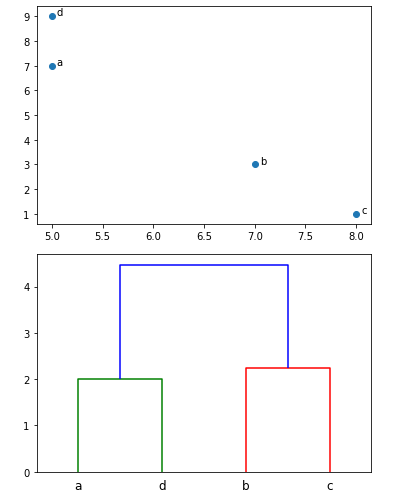
\includegraphics[width=.6\linewidth]{figs/deno/toy-dendrogram.png}
  \caption{Top: A simple scatter plot of some arbitrary data points 
  \newline Bottom: A dendrogram illustrating the agglomerative process. 
  \newline Notice that $(b,c)$ are merged after $(a,d)$ indicating that latter are more similar}
  \label{fig:toy-dendrogram}
\end{figure}

 
Under hierarchical clustering, any number of final clusters can be set. 
This means that the number of final clusters is determined up to human discretion, thereby not guaranteeing clearly defined clusters.

 
\subsection{Evaluating Clusters}
 After the clusters have been generated, it is useful to evaluate the result.
%  well the observations have been grouped. 
One way to do this is with the Davis-Bouldin index (DB-index or DB-criterion) is defined as the ratio of the “within-cluster”-distance and “between-cluster”-distance. “Within-cluster”-distance is a description of dispersed elements of a cluster is and “between-cluster”-distance  is a description of how far apart the cluster are from each other. This means that a low DB-index is an indication of a good clustering result. 

In the context of this, the information gained from the DB-index is minimal.
This is because it as well as all other numerical evaluations,  depend on a ground truth of how to correctly quantify the similarity distance. 
The index may provide some insight, however, we expect the true information gain to be minimal and its ranking to be biased.


As a closing remark, we acknowledge that there is no general standard for what constitutes a “reasonable clustering” on account of it being highly domain-dependent.
Human inspection remains a vital tool for evaluating final clusterings\cite{79-SilhouetteAnalysis}. 
In order to discuss the clustering results from a visual perspective, we define the terms \textit{Fuzzy} and \textit{Crisp} as seen in \Cref{def:cluster_defs_fuzz,def:cluster_defs_cri}.

\begin{definition}\label{def:cluster_defs_fuzz}
A cluster is \textbf{fuzzy} if its members appear spread out and with seemly little relation to each other.  
For a "good" clustering result, we wish to minimize the number of fuzzy clusters. 

\end{definition}

\begin{definition}\label{def:cluster_defs_cri}
A cluster is \textbf{crisp} if its members create a clear silhouette with seemly a clear correspondence.
For a "good" clustering result, we wish to have as many crisp clusters as possible 
\end{definition}
